% fig_threshold.tex
% Adaptive threshold I_thr vs I_rest (TR-17)
% Law: I_thr = max(0.08, 0.15 * I_rest)
% Security margin = I_thr / (0.005 * I_rest) -- always >= 30x at I_rest > 0.5
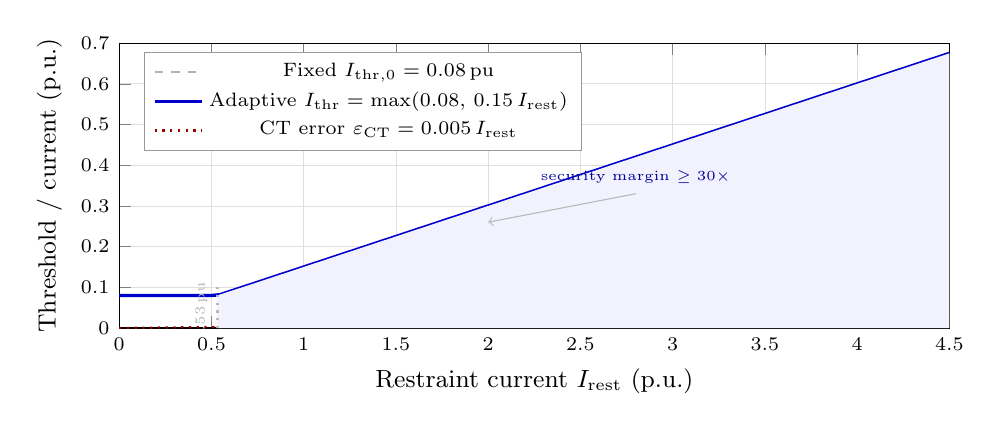
\begin{tikzpicture}
\begin{axis}[
  width=\columnwidth, height=5.2cm,
  xlabel={Restraint current $I_{\rm rest}$ (p.u.)},
  ylabel={Threshold / current (p.u.)},
  xmin=0, xmax=4.5,
  ymin=0, ymax=0.70,
  xtick={0,0.5,1,1.5,2,2.5,3,3.5,4,4.5},
  ytick={0,0.1,0.2,0.3,0.4,0.5,0.6,0.7},
  grid=both,
  grid style={gray!25,line width=0.3pt},
  tick label style={font=\scriptsize},
  label style={font=\small},
  legend style={at={(0.03,0.97)},anchor=north west,
                font=\scriptsize,fill=white,draw=black!40},
  clip=true]

  % Fixed threshold (baseline)
  \addplot[gray!60,thick,dashed,domain=0:4.5] { 0.08 };
  \addlegendentry{Fixed $I_{\rm thr,0}=0.08$\,pu}

  % Adaptive threshold
  \addplot[blue!80!black,very thick,samples=100,domain=0:4.5]
    { max(0.08, 0.15*x) };
  \addlegendentry{Adaptive $I_{\rm thr}=\max(0.08,\,0.15\,I_{\rm rest})$}

  % CT error curve (0.5% of I_rest)
  \addplot[red!60!black,thick,dotted,domain=0:4.5]
    { 0.005*x };
  \addlegendentry{CT error $\varepsilon_{\rm CT}=0.005\,I_{\rm rest}$}

  % 30x margin annotation region fill
  \addplot[fill=blue!5,draw=none,forget plot,domain=0.53:4.5]
    { max(0.08, 0.15*x) } \closedcycle;

  % Knee point annotation
  \draw[gray!55,dotted,thick]
    (axis cs:0.533,0) -- (axis cs:0.533,0.10)
    node[above,font=\tiny,gray!55,rotate=90,pos=0.4]{$0.53$\,pu};

  % 30x margin annotation
  \node[font=\tiny,blue!60!black]
    at (axis cs:2.8,0.37) {security margin $\geq 30\times$};
  \draw[->,gray!55]
    (axis cs:2.8,0.33) -- (axis cs:2.0,0.26);

\end{axis}
\end{tikzpicture}
